\chapter{Generators in Peachpie}

The goal of this thesis is to enable Peachpie compiler to handle PHP generator methods while keeping as much of their original semantics as possible. That means we do not want to change their behavior and want to enable all the features they offer in PHP, only now compiled to CIL and executed either by the CLR or another CLI environment.
 
As noted in previous chapters\footnote{Chapter \ref{sec:3:1}}, this in itself is complicated, because unlike the PHP runtime Zend Engine, the CIL and CLR do not have a native support for generators or generally pausing the execution of a method at arbitrary points. Also, almost all other CIL based languages with generators, such as C\# or F\#, that implement them by compiler transformations have them in a substantially more limited form than PHP.

Other than that, we also want to reuse existing Peachpie infrastructure and only implement generator specific bits when necessary. While this goal is not as important for our immediate work, it is necessary for the project as a whole. Cluttering the compiler with logic for a feature that is not actually used as often would simply be inexcusable.

\section{Basic generators implementation}

Before dealing with all the complexities of PHP’s generators, let us first explore how an implementation of their limited subset would work within Peachpie. Specifically, we will ignore \emph{yield} in exception handling blocks and expect it to be only in places where it could happen as a statement, i.e. no \emph{yield} inside an expression tree, for this chapter. 

Much like Roslyn’s approach, our implementation of generators within Peachpie will also be based on transforming the original generator method into an iterator's \emph{next} method. So as not to repeat ourselves, we will only point out the differences in the next section.

\subsection{Iterator object}

Unlike in C\#, where generator methods are free to return any object implementing an \emph{IEnumerator} interface, the PHP specification dictates that the returned object must be an instance of a \emph{Generator} type \citep{GenPHP, GenPHPRFC}. This means that in Peachpie we cannot just synthesize a new type for each generator method as Roslyn does.

If we were to do that, all reflection methods and type checks would report the actual synthesized type on the returned iterator instance instead of the \emph{Generator} type, as required by PHP’s specification . We could theoretically hard code exceptions for these synthesized types into all methods that query an instance’s type, but that would go against our goal to implement as little feature specific code as possible.

Instead, we must create one generator type in Peachpie’s runtime library and use it as a basis for all generator methods to return. That approach, however, carries some limitations with it. The generator type can now include only shared code and fields. That means neither a specific \emph{next} method’s implementation nor fields for lifted local variables from said method.

Other than that, the \emph{Generator} type can be practically the same as the ones synthesized by Roslyn as it is a simple implementation of PHP's \emph{Iterator} interface (\autoref{list5.1:GeneratorType}). It can hold a captured reference to the \emph{this} instance of the original generator method, a state field to know what point the \emph{next} method should continue from,  fields for the \emph{current} element and, since we are in PHP now, its \emph{key}.

\begin{listing}[H]
\caption{Simplified version of the Generator type.}
\label{list5.1:GeneratorType}
\begin{minted}{csharp}
public delegate void GeneratorStateMachineDelegate(
  Context ctx, object @this, PhpArray locals, 
  Generator gen);
public class Generator : Iterator
{
  readonly Context _ctx;
  readonly GeneratorStateMachineDelegate _stateMachineMethod;
  readonly object _this;
  readonly PhpArray _locals;
  internal int _state = 0;
  internal PhpValue _currValue, _currKey;
  public void next() =>
  _stateMachineMethod.Invoke(_ctx, _this, _locals, gen: this);
}
\end{minted}
\end{listing}

\subsection{Next method implementation and local variables}

The \emph{next} method's implementation problem is easily solvable. The shared generator type can hold a delegate to an implementation of the \emph{next} method instead of the method itself. This enables Peachpie compiler to synthesize the \emph{next} method anywhere and then to assign its delegate to the generator. The generator must still implement some \emph{next} method to comply with the Iterator interface but it can be a shim that only calls the saved delegate.

There is only one restriction with regards to the actual \emph{next} method’s placement. The transformed method must be accessible from within the original generator method. The reason is that the original method is where the instantiation and initialization of the generator, thus also the creation and assigning of the delegate, happens. 

One such suitable place is the enclosing type of the original method, where it can always be synthesized as a static method. It being a static method is not a problem because, as mentioned in the chapter about Roslyn’s implementation, a reference to the enclosing type’s instance is passed as a \emph{this} parameter. And since the enclosing type could be a static class, it cannot be a normal instance method anyway.

The inability to add fields to the generator type can also be overcome. As described in the CIL emit phase chapter\footnote{Chapter \ref{CodeGen}}, Peachie's \emph{CodeGenerator} supports specifying where local variables should live within a method with the option to, for example, move them to a \emph{PhpArray}.

With that, a \emph{PhpArray} field can be added to the generator type and we can specify that all of the \emph{next} method's local variables should live on it. Because parameters are considered local variables in Peachpie, this approach handles them as well. They only need to be initialized with their values in the original generator method. That way, the \emph{next} method’s local variables and parameters get lifted to the generator type the same way as in Roslyn, with the only difference being that they do not get lifted to individual fields but to a single \emph{PhpArray} (\autoref{fig5.1:Generator}).

\subsection{Accessibility of fields on the Generator type}

Moving the \emph{next} method outside of the generator type means that the method cannot access its fields such as \emph{current} or state directly through a \emph{this} reference. That is a problem, because the method needs to both read and write these fields to progress the generator. An effective solution is to pass the generator instance as a parameter through the \emph{next} method delegate - in essence to not only call the delegate from within the generator’s own \emph{next} method, but to call it with a \emph{this} reference as a parameter.

That on its own would be enough if all the fields on the generator type were public. That is, however, not our objective. We want the generator type to have the same public API as it does in PHP and there are no such public fields in PHP’s \emph{Generator}. Therefore, we need to find a way to access the fields from a method within the user’s assembly, the transformed \emph{next} method the generator has a delegate to, without having to make the fields accessible to other user code.

One way to do this is to make the generator fields internal and create public getter and setter methods for these fields in the Runtime library. Since the generator type also lives there, the methods can access its fields and, because they are public, they can be used from within the synthesized \emph{next} method (\autoref{fig5.1:Generator}). The methods can be simple static getters and setters, always taking a generator instance as a first parameter and either returning an appropriate field’s value or taking its value as a second parameter and then setting it on the instance.

\begin{figure}[h]
	\centering	
	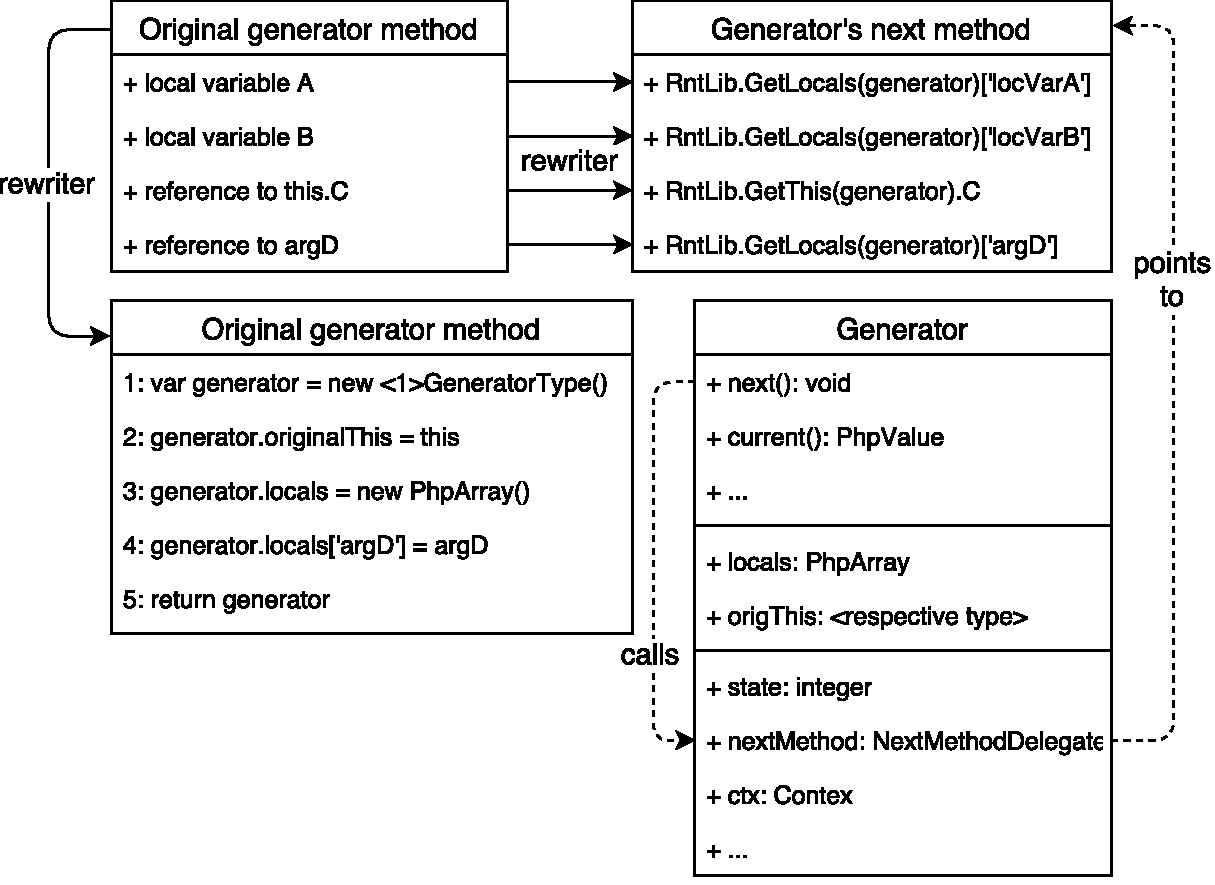
\includegraphics[scale=0.70]{../img/5_1_Generator}	
	\caption{Transformation of the generator method.}
	\label{fig5.1:Generator}
\end{figure}

While it is true that this approach still opens a way for the user to modify the generator’s internal state, it has to be done through special methods from Peachpie runtime library and as such, it can hardly be done by accident. It also ensures a compliant public API of the \emph{Generator} type.

\subsection{Context handling}

Being in PHP, we need to ensure that the correct PHP \emph{Context} gets passed to our moved \emph{next} method. There are two ways to do it. Current \emph{context} can either be passed as part of each call to the generator methods, and subsequently via a delegate to the \emph{next} method, or it can be captured once during the generator’s initialization and then reused the same way as is the \emph{this} instance.

Neither approach is inherently wrong. Passing the \emph{context} with each call ensures the current one is used even in situations where one generator instance is used with multiple PHP \emph{context}s. That can happen, for example, when PHP code is called from some other .NET language and multiple \emph{context}s are created manually. This approach is also more in line with how \emph{context} on normal instances is handled. It is not captured in the constructor and then used by all the instance methods, but always passed as a parameter.

On the other hand, capturing the \emph{context} on the generator’s creation better represents the idea that the generator is a fully self-contained object. It is also marginally easier to implement and provides better opportunities for interop between PHP generators and other .NET languages. This way, a generator can be created in PHP and then used elsewhere as a normal iterator, without having to explicitly keep and supply its \emph{context}. Thus, the capture once in the original generator method approach was chosen.

\subsection{Rewriter}

Due to architectural differences, we will not have a standalone rewriter component in Peachpie. While it would be possible, there are, as of writing this thesis, no other candidates that could make use of them within the compiler. And adding a generic support just to have one rewriter for generators goes against our goal to keep the implementation as simple as possible. Instead, our implementation will rely on support by the \emph{SemanticBinder}, slightly changed emit of a \emph{MethodSymbol} and \emph{StartBlock}\footnote{Chapter \ref{StartBlock}}, and a new semantic node. 

As long as we limit ourselves to \emph{yield} only at places where it could be as a statement, which is the temporal restriction we have set for this chapter, the support provided by the \emph{SemanticBinder} can be minimal. It needs to do two things: bind the new semantic object - \emph{BoundYieldExpression} - when it encounters the AST’s \emph{YieldExpression} and mark the method’s symbol as a generator. 

\subsection{Bound yield expression}

The \emph{BoundYieldExpression} can be a rather simple semantic node with two children: the yielded key and yielded value expressions. It should generate CIL to set the yielded key and value fields on the generator instance, update its state, \emph{return}, and mark a label for the subsequent continuation (\autoref{fig5.1:Rewriter}). 

Due to being an expression, albeit for this chapter limited to places where it could also be a statement, it needs to push and leave its value on the evaluation stack. However, since its value will not be needed due to our restriction, it can just as well be an empty \emph{PhpValue}. The value will always get discarded, anyway. The restriction also handles the problem that we are emitting a \emph{return} from within an expression, i.e. in a situation in which the evaluation stack might not be empty.

It is true that all of the \emph{BoundYieldExpression} could be replaced with a number of normal PHP statements by lowering. That would, however, require the \emph{SemanticBinder} to be able to produce multiple semantic statements for only one AST node, and for the \emph{BuilderVisitor} to accept them. And while such support could be added, it was decided that it would be too complex.

\begin{figure}[h]
	\centering	
	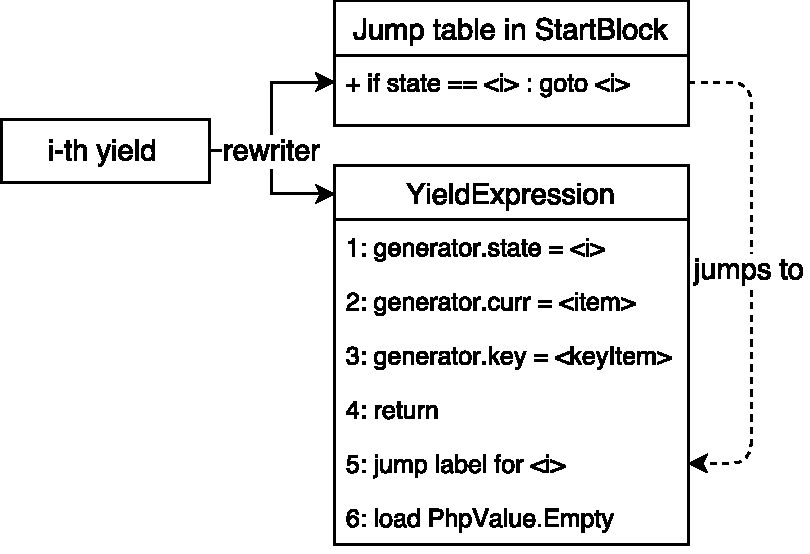
\includegraphics[scale=0.75]{../img/5_1_rewriter}	
	\caption{Rewrite of a yield expression.}
	\label{fig5.1:Rewriter}
\end{figure}


\subsection{Start block}\label{StartBlock}

The \emph{StartBlock} is a special instance of a \emph{BoundBlock} that is present in the beginning of each method’s control flow graph (\autoref{fig3.4:EmitOrder}). As such, its emit routine is the perfect place to generate a jump table for generator methods. It can, when its enclosing method symbol is a generator, query all present \emph{yield} statements that were previously set by, for example, the semantic binder and generate the whole jump table.

\subsection{Method symbol}

The method symbol’s emit must be changed as well. When it represents a generator, it cannot simply generate the CIL representation of its body. If it did that, it would not produce a method that returns an iterator as it should, but a method that implements the iterator’s \emph{next} method.

Instead, three things need to happen. First, a new static method representing the generator’s \emph{next} method must be synthesized in the enclosing type. Second, the original body needs to be emitted inside the synthesized method with its \emph{CodeGenerator} set to offload local variables into a generator’s locals field. As explained earlier, the synthesized \emph{next} method accepts a \emph{Generator} as a parameter.

Third, a sequence of statements that create, initiate, and \emph{return} a \emph{Generator} instance must be emitted as the actual current MethodSymbol’s body, producing a method that returns an iterator. As part of the initiation phase a delegate to the synthesized \emph{next} method must get created and assigned to the newly constructed generator instance. Also, values of all parameters need to get copied to the generator’s locals array, as previously discussed.

\section{Yield as an expression - theory}

With that, we have described a design of a generator’s compilation within the Peachpie platform with a featureset limited to more or less C\# generators. Now, let us broaden it with the support for \emph{yield} as an expression. Before going into details on the specific implementation, let us first take a look at the general idea behind our approach. 

As said before, a \emph{yield} being an expression is a problem, because an expression can happen in a situation where the CIL evaluation stack might not be empty. Since \emph{yield}s include a \emph{return} and returning with a non-empty evaluation stack is forbidden, it does not go well together. Even if it were allowed, there would still be the problem that the non-empty evaluation stack would represent some sort of state - one that would need to get saved and then retrieved upon the continuation.

\subsection{Possible approaches}

Fundamentally, there are two possible ways to approach this problem. One can either come up with a mechanism to save and then retrieve the evaluation stack or rearrange the semantic graph so that \emph{yield}s are only in places where they could happen as statements.

While the first approach might be appealing, after all it more closely mimics the Zend Engine’s way of handling yields\footnote{Chapter \ref{ZendGen}}, it is almost impossible to implement. Because the CIL does not have any instructions to query the contents or to completely save/load the evaluation stack, the compiler would have to do it manually. That means it would have to track the stack’s content throughout the compilation and then emit individual instructions to save/load its content, one element at a time.

That would mean two things. First, we would either have to create our own version of the \emph{CodeGenerator} that would be able to keep track of what the evaluation stack contains at any moment or we would have to change the emit of each semantic node to save the information about what it puts on the stack explicitly. Both of these would be relatively complex to do and, in case of the second approach, even to maintain due to possible new semantic nodes. Second, either of them would mean an increase in memory usage because we would need to remember information previously not required, all of which just to support only a \emph{yield} as an expression. 

On the other hand, the second approach, to rearrange the semantic tree, requires only a few local implementation changes and does not cause a substantial memory consumption increase. Essentially, it is based on the idea that we can break an expression tree into a series of statements while keeping the meaning and order of execution the same.

\subsection{Branch capture \& yield splitting}

There are two important observations required for this method. First, a yield can be broken into two semantic nodes. A statement that does the value and key setting, state saving, \emph{return}, and marking the continuation label, acting as the equivalent of a C\# \emph{yield} statement. The other node is an expression that represents the sent value. If the expression directly follows the statement, the result is, in terms of emitted CIL, the same as with one combined yield expression (\autoref{fig5.2:Splitting}). 


\begin{figure}[h]
	\centering	
	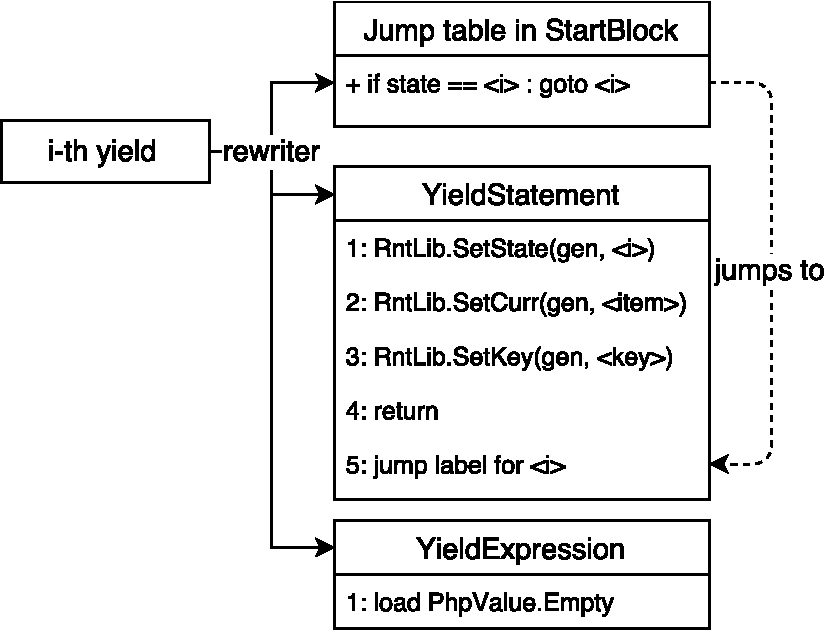
\includegraphics[scale=0.75]{../img/5_2_yieldSplitting}	
	\caption{Splitting of a yield into an expression and a statement.}
	\label{fig5.2:Splitting}
\end{figure}

Second, we can cut any branch from an expression tree and prepend it before the tree while keeping the meaning of the program the same except for the order of execution. To do it, we need to create a temporal variable, replace the branch in the tree with a read from said variable, and prepend the tree with a statement that assigns the branch that was replaced to the variable it was replaced with (\autoref{fig5.2:CaptureBranch}). Let us call this process capturing a branch.

The problem with the order of execution is that the captured branch, being lifted to the prepended statement, will get executed before any other expression from the tree. Even before all the expressions in branches that might be to the left of the captured branch and that were therefore supposed to be executed first. In the figure below, the expressions $5$ and $6$ respectively will get executed first, even though they should come after expressions $1$, $2$, $3$, and $4$.


\begin{figure}[h]
	\centering	
	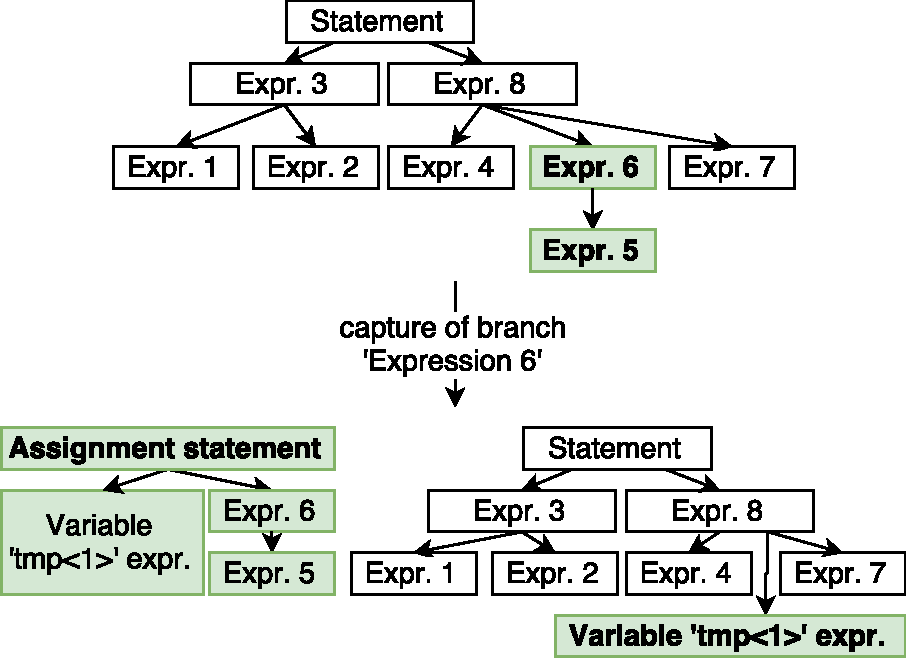
\includegraphics[scale=0.75]{../img/5_2_capturing}	
	\caption{Capturing a sole branch.}
	\label{fig5.2:CaptureBranch}
\end{figure}

An obvious solution to this problem is to cut and prepend not only the one branch we want to capture, but also, in their respective order from left to right, all other branches that are supposed to get executed before it (\autoref{fig5.2:CaptureAllBranch}). Since the semantic graph emit, and thus also the execution, follows a post-order traversal, we must cut and prepend all branches that are higher and to the left of the branch we want to capture. 

To be specific, that includes all branches that start to the left of the path between the root of our captured branch and the root of the whole semantic graph. The reason lies in a post-order traversal of the semantic graph. 

It starts with the graph’s root. Then it goes through the root’s leftmost child, followed by its next child, and so on. Let us say, for example, that the second element of our aforementioned path is the root’s third child. When the traversal enters it after going through the branches started by the root’s first two children, it goes into its leftmost child first, again. It then continues the same way until it encounters the root of our branch. When that happens, it keeps following the same logic, traversing the whole branch before closing its root and starting to visit any other nodes. After the traversal is finished with the branch, it closes its root and goes one level up, starting to traverse the branch’s root’s first sibling to the right.   

All other expressions, be it those directly on the path or on branches to the right, are supposed to be evaluated after our branch and, as such, do not have to be cut and prepended. The ones on the path have our branch among their children and thus need its result - our branch - to be evaluated first. And the ones on the right need to be evaluated later, simply because of post-order traversal rules. 

\begin{figure}[h]
	\centering	
	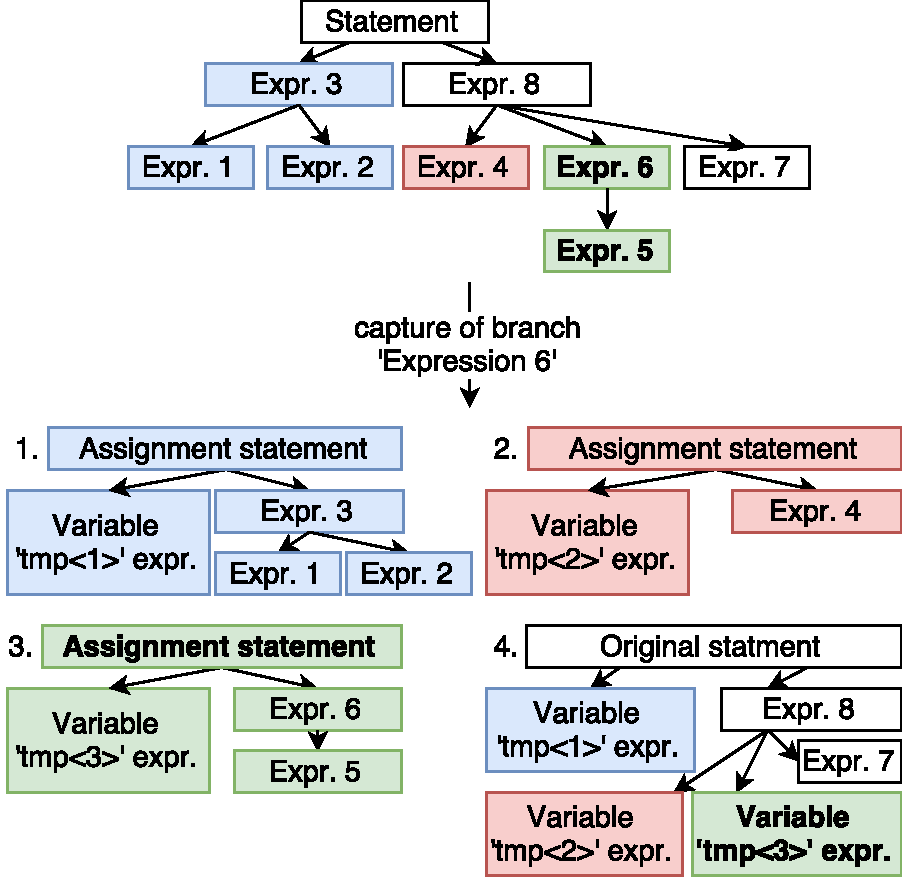
\includegraphics[scale=0.75]{../img/5_2_captureAllOnPath}	
	\caption{Capturing a whole branch while maintaining execution order.}
	\label{fig5.2:CaptureAllBranch}
\end{figure}

\subsection{Semantic tree transformation}

\begin{figure}[h]
	\centering	
	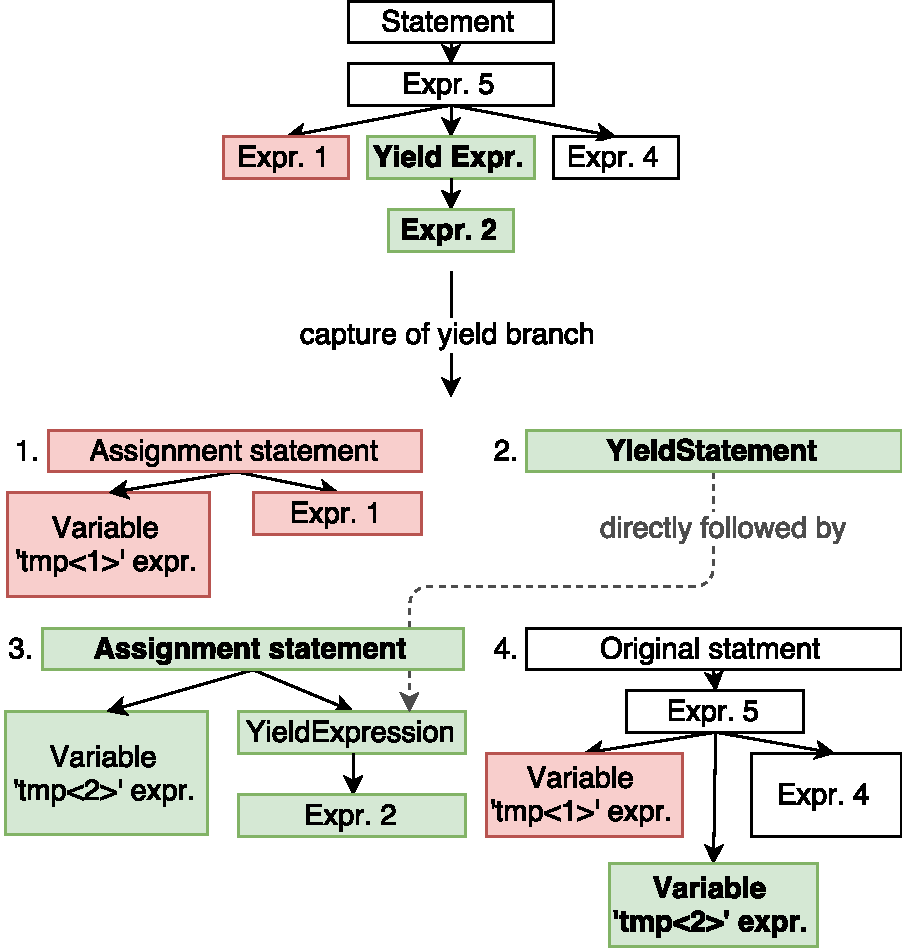
\includegraphics[scale=0.75]{../img/5_2_yieldCapturing}	
	\caption{Capturing a whole branch starting with a yield.}
	\label{fig5.2:CaptureYield}
\end{figure}

\subsection{Short circuit evaluation}

\begin{listing}[H]
\caption{Conditional expression whose captured branch is not conditioned.}
\label{list5.3:CondNotGuarded}
\begin{minted}{php}
<?php
// original expression before capturing the yield branch
$result = isTrue() ? yield 0 : “falseValue”;

$tempBranchResult = yield 0;
$result = isTrue() ? $tempBranchResult : "falseValue";
\end{minted}
\end{listing}

\begin{listing}[H]
\caption{Conditional expression whose condition is evaluated twice.}
\label{list5.3:CondTwice}
\begin{minted}{php}
<?php
if (isTrue()) { $tempBranchResult = yield 0; }
$result = isTrue() ? $tempBranchResult : "falseValue";
\end{minted}
\end{listing}

\begin{listing}[H]
\caption{Conditional expression captured correctly.}
\label{list5.3:CondCorrect}
\begin{minted}{php}
<?php
$tmpResult = isTrue();
if ($tmpResult) { $tempBranchResult = yield 0; }
$result = $tmpResult ? $tempBranchResult : "falseValue";
\end{minted}
\end{listing}

\section{Yield as an expression - implementation}

\subsection{Binding multiple elements}

\begin{figure}[h]
	\centering	
	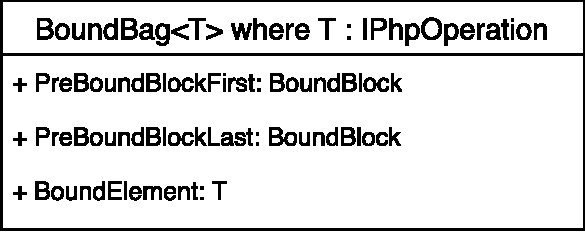
\includegraphics[scale=0.75]{../img/5_3_BoundBag}	
	\caption{Bound bag.}
	\label{fig5.3:BoundBag}
\end{figure}

\begin{figure}[h]
	\centering	
	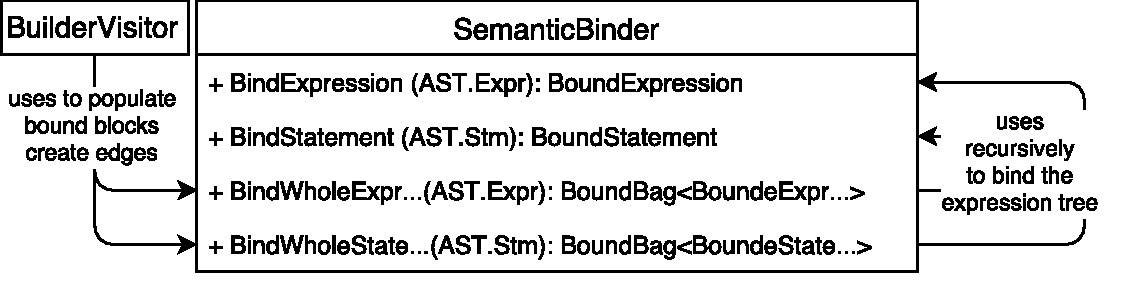
\includegraphics[scale=0.75]{../img/5_3_BoundWholeExpression}	
	\caption{Builder visitor's and semantic binder's relationship.}
	\label{fig5.3:BindWholeExpr}
\end{figure}

\begin{figure}[h]
	\centering	
	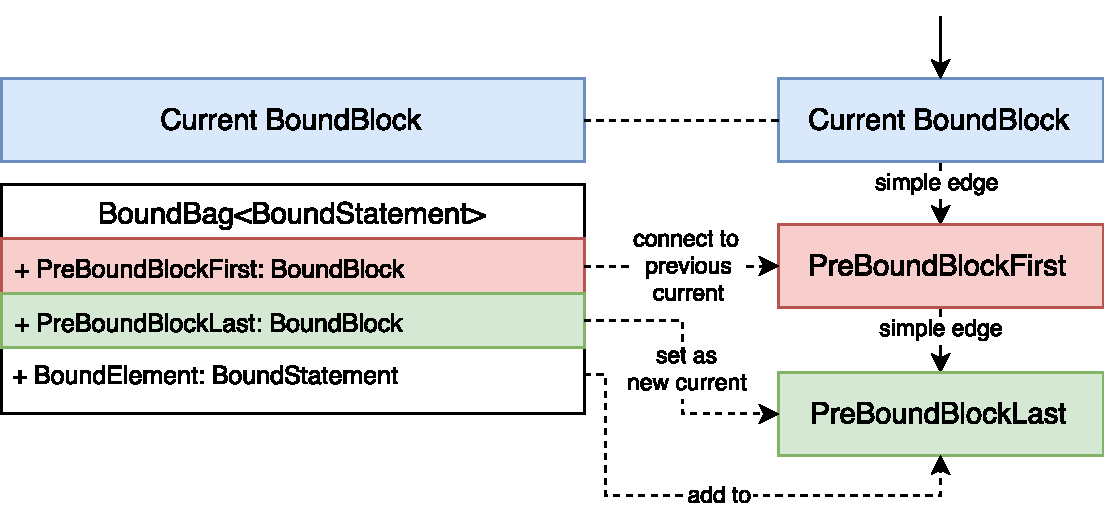
\includegraphics[scale=0.75]{../img/5_3_newStatement}	
	\caption{Connecting a bound bag as a new statement.}
	\label{fig5.3:BindNewStm}
\end{figure}

\begin{figure}[h]
	\centering	
	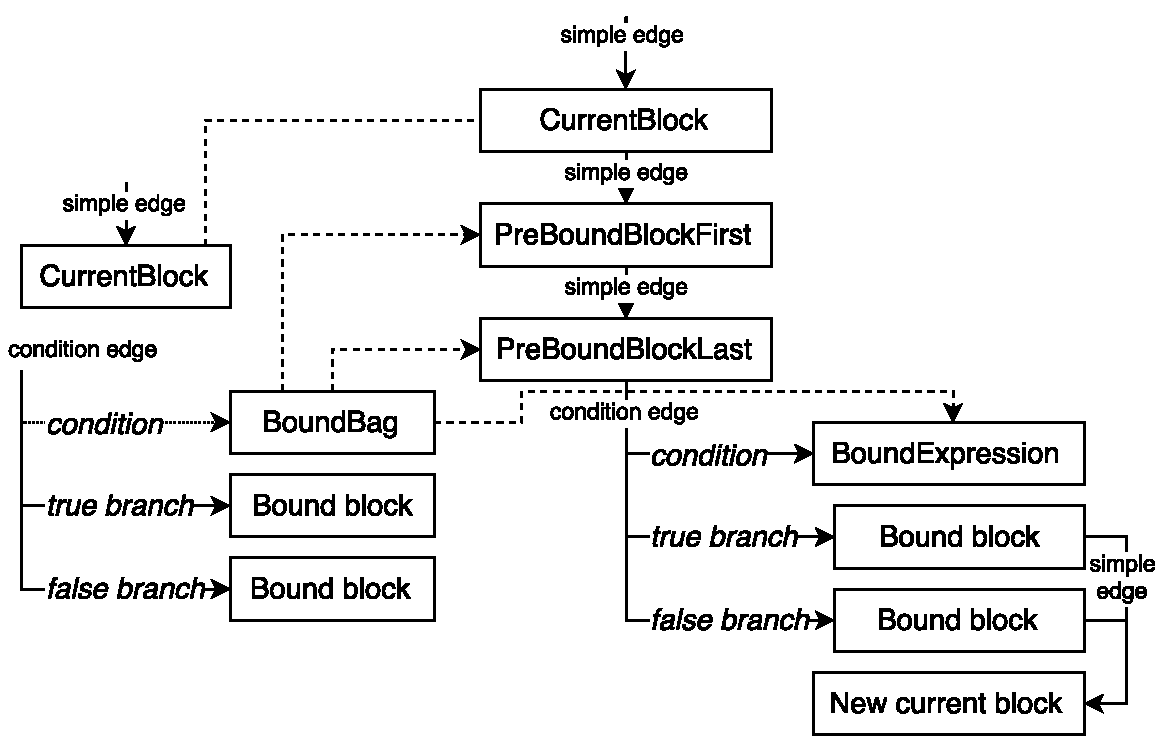
\includegraphics[scale=0.70]{../img/5_3_newInIfEdge}	
	\caption{Connecting a bound bag as a condition edge's condition.}
	\label{fig5.3:BindIfEdge}
\end{figure}

\begin{figure}[h]
	\centering	
	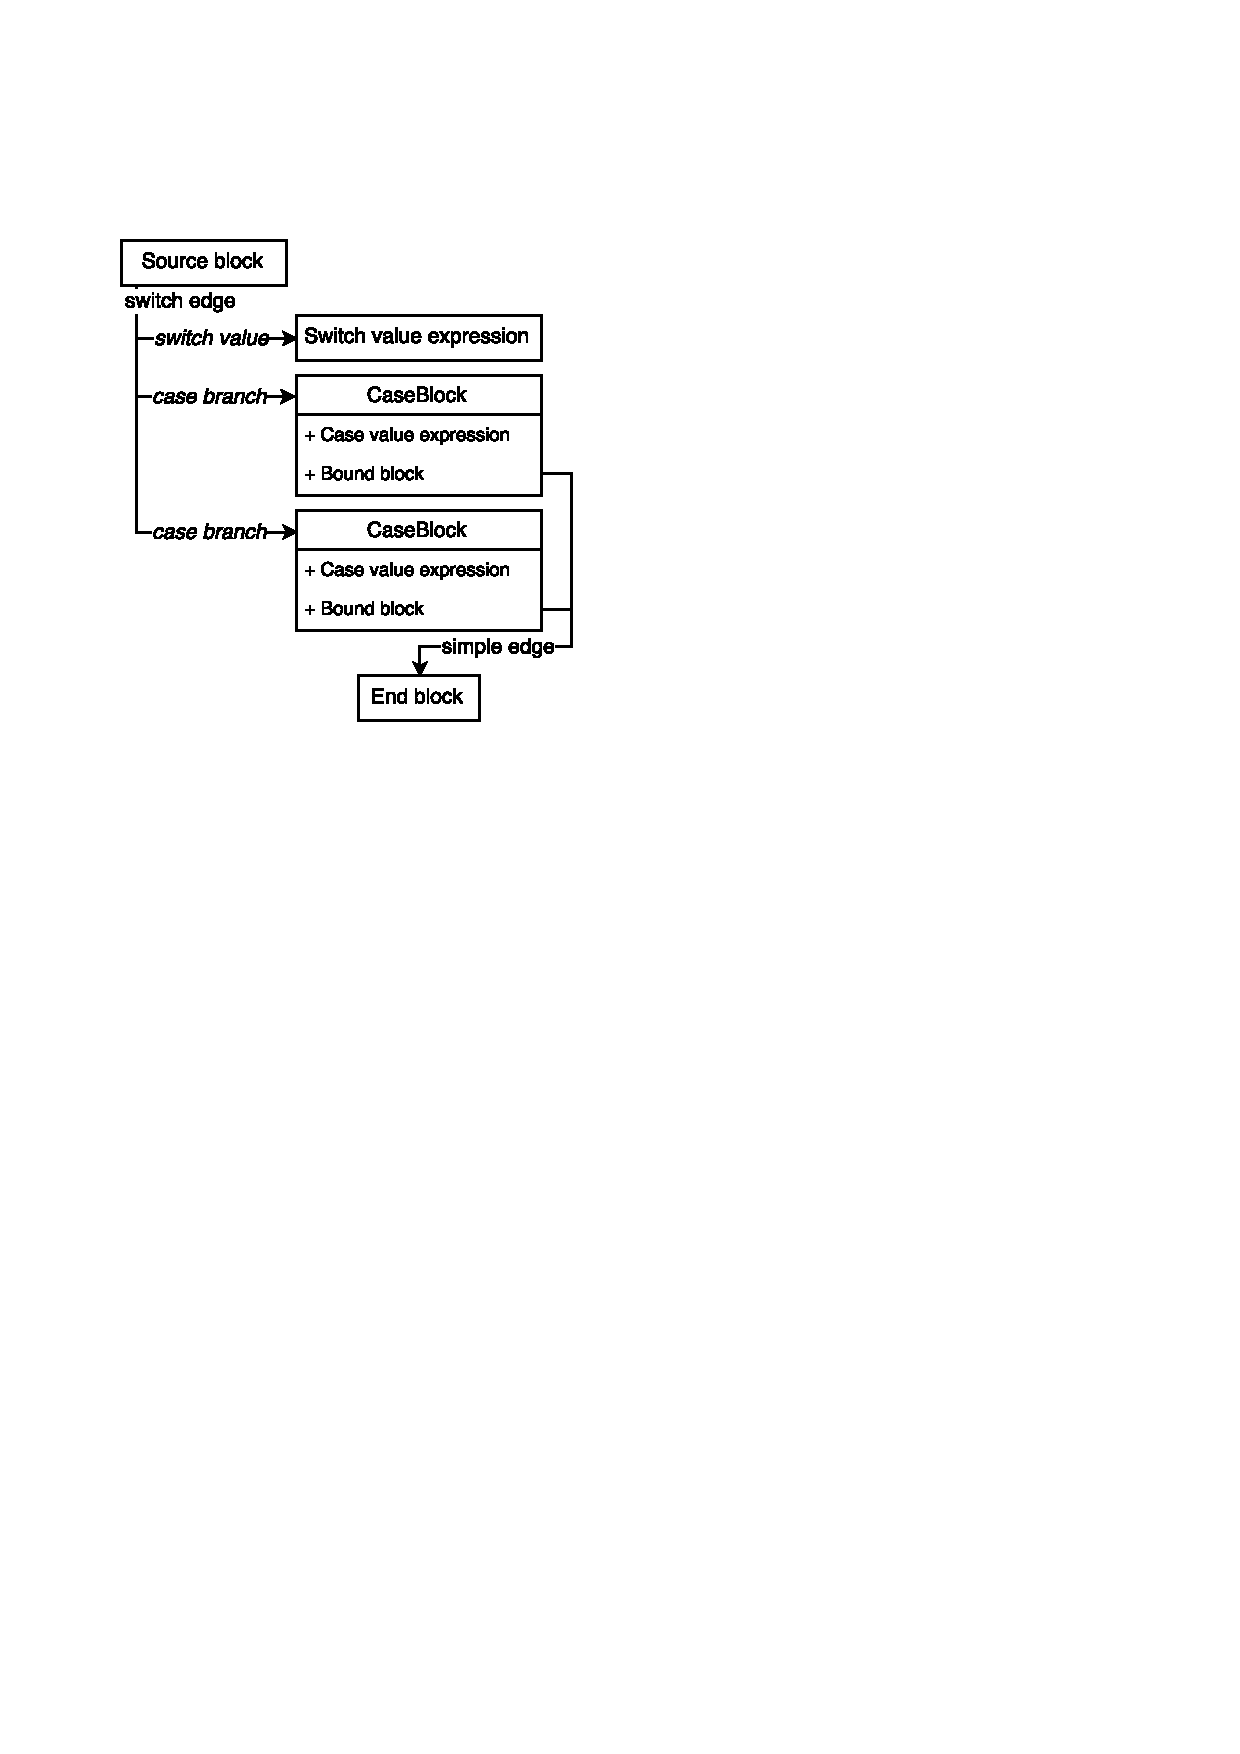
\includegraphics[scale=0.75]{../img/5_3_switchEdge}	
	\caption{Switch edge diagram.}
	\label{fig5.3:SwitchEdge}
\end{figure}

\subsection{Capturing branches with yields}

\begin{figure}[h]
	\centering	
	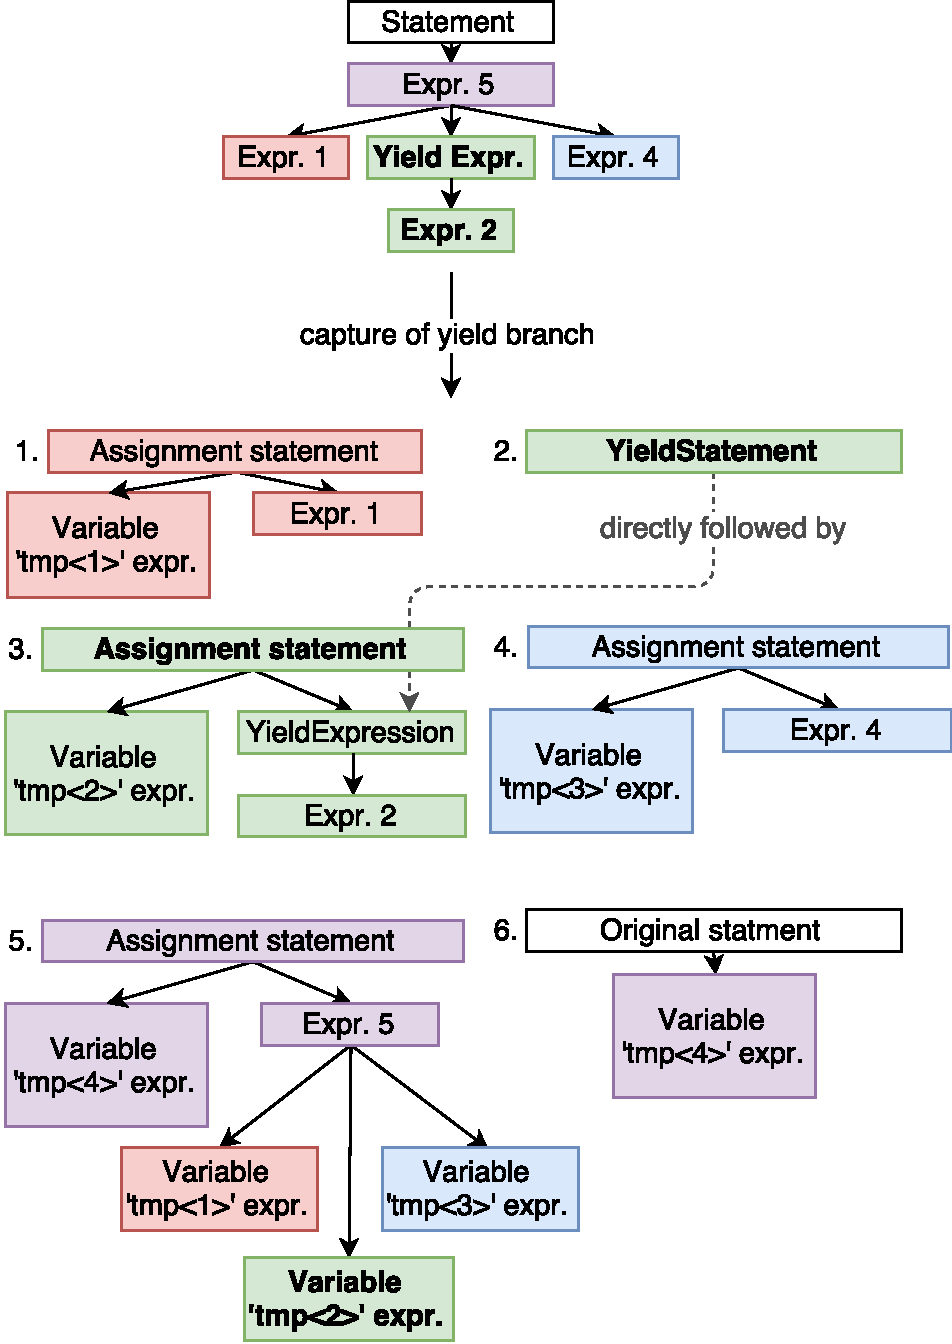
\includegraphics[scale=0.75]{../img/5_3_branchesWithYields}	
	\caption{Capturing a branch with a yield.}
	\label{fig5.3:CaptureWithYield}
\end{figure}

\subsection{Correctness of modified capturing algorithm}

\subsection{Creating and keeping the pre-bound graph}

\begin{figure}[h]
	\centering	
	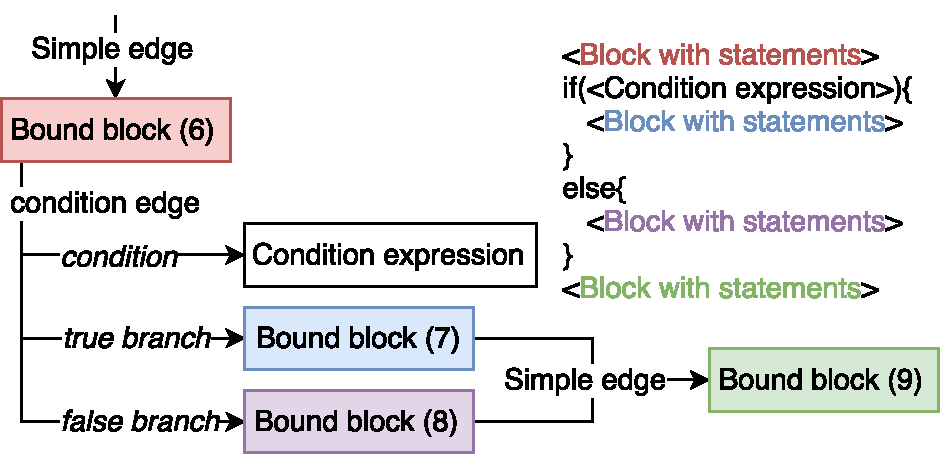
\includegraphics[scale=0.75]{../img/5_3_blockOrdinal}	
	\caption{Ordinal number of bound blocks.}
	\label{fig5.3:BlocksOrdinal}
\end{figure}

\subsection{Path between the root and yields}

\begin{figure}[h]
	\centering	
	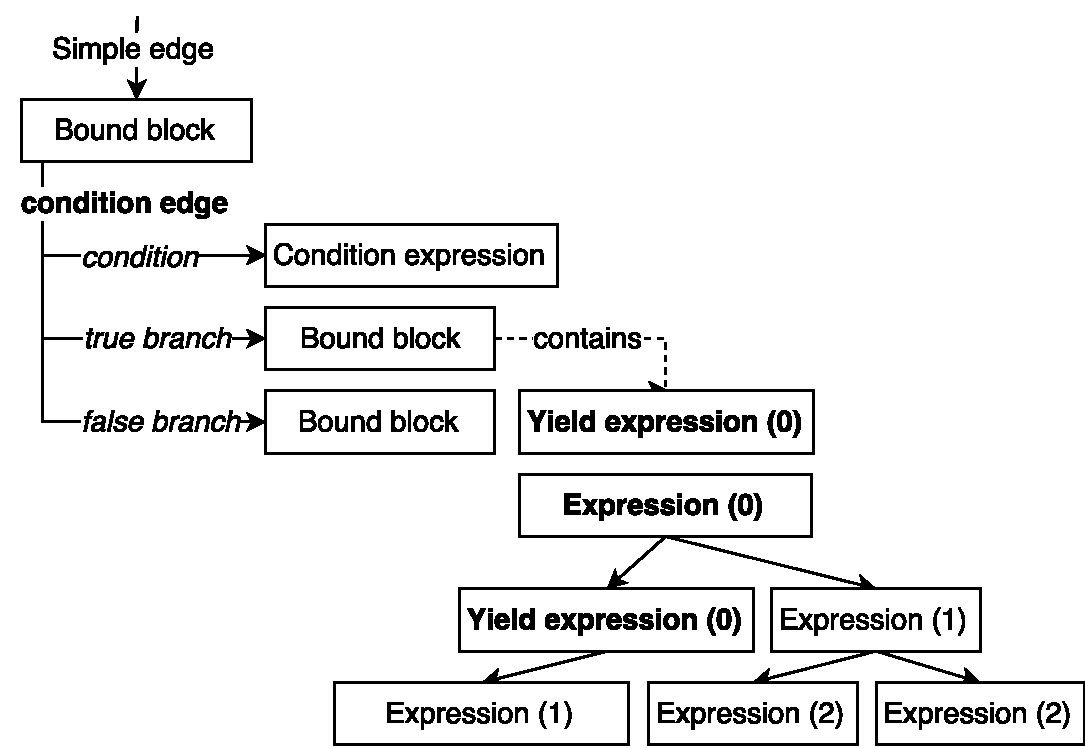
\includegraphics[scale=0.75]{../img/5_3_path}	
	\caption{Path between a yield and expression tree's root.}
	\label{fig5.3:Path}
\end{figure}

\subsection{Conditioned branches}

\begin{figure}[h]
	\centering	
	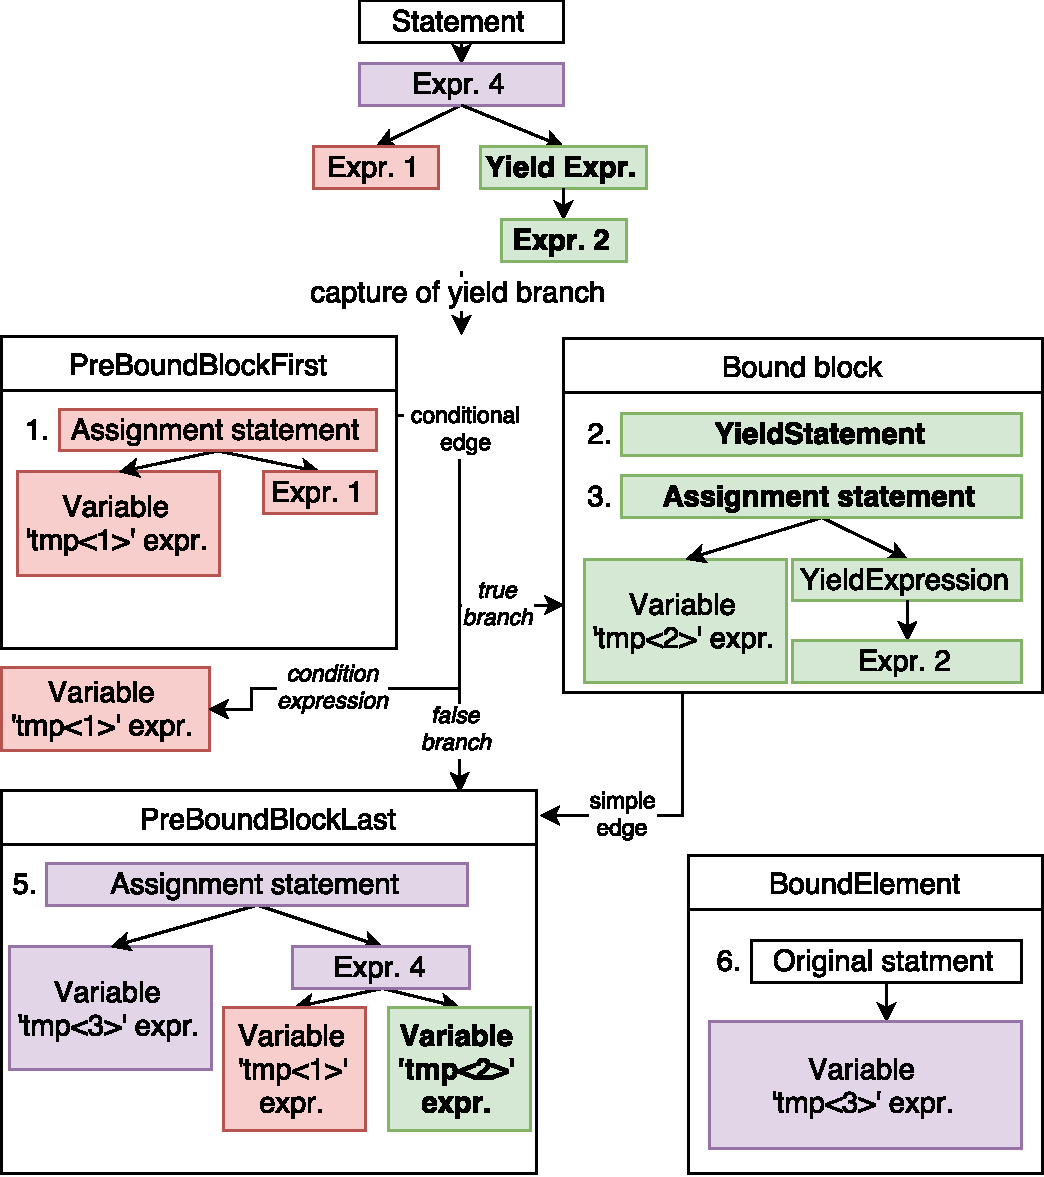
\includegraphics[scale=0.75]{../img/5_3_yieldInCond}	
	\caption{Capturing a yield in a conditioned branch.}
	\label{fig5.3:YieldInCond}
\end{figure}

\subsection{Implementation remarks}

\section{Yield in exception handling blocks}

\subsection{Yields and exception handling blocks in PHP}

\subsection{Solution in Peachpie}

\section{Future work}

\begin{figure}[h]
	\centering	
	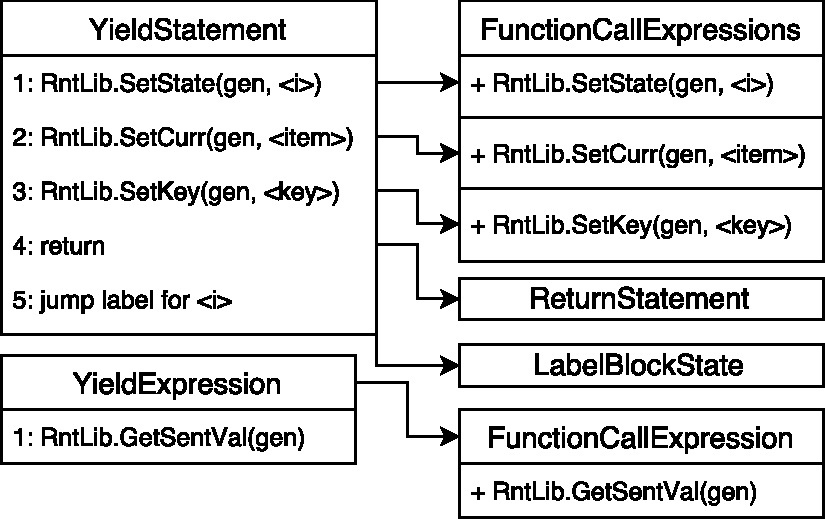
\includegraphics[scale=0.75]{../img/6_6_yieldLowering}	
	\caption{Possible lowering solution to a yield expression and a yield statement.}
	\label{fig5.5:YieldInCond}
\end{figure}

